\documentclass[11pt]{article}
\usepackage[margin=0.9in]{geometry}
\usepackage{amsmath,amssymb}
\usepackage{booktabs}
\usepackage{graphicx}
\usepackage[colorlinks=true,linkcolor=blue,citecolor=blue,urlcolor=blue]{hyperref}
\usepackage{xcolor}
\usepackage{tikz}
\usetikzlibrary{arrows.meta,positioning,fit,backgrounds,calc}
\usepackage{enumitem}
\setlist{nosep}

\definecolor{frozengray}{HTML}{6B7280}
\definecolor{trainedblue}{HTML}{2563EB}
\definecolor{geogreen}{HTML}{059669}
\definecolor{froz}{HTML}{F3F4F6}
\definecolor{trai}{HTML}{DBEAFE}
\definecolor{geob}{HTML}{D1FAE5}
\newcommand{\metric}{AP$_{50}^{\text{axis+origin}}$}
\newcommand{\apfifty}{AP$_{50}$}

\title{\vspace{-8mm}Articulate3D Challenge --- Technical Report\\
\large Frozen USDNet, Geometric Priors, and Structural Post-Processing}
\author{Junyuan Fang}
\date{September 2026}

\begin{document}
\maketitle
\vspace{-6mm}

\section*{Team}
\begin{tabular}{@{}lll@{}}
\toprule
Name & Affiliation & Email \\
\midrule
Junyuan Fang & Independent Researcher & \texttt{fangjunyuan1@gmail.com} \\
\bottomrule
\end{tabular}

\smallskip
\noindent Final standing (boards frozen 2026-08-28): \textbf{1st} on Movable-dev (\metric{} $=0.5038$) and Interaction-dev (\apfifty{} $=0.6446$);
\textbf{2nd} on Movable-test ($0.4056$) and Interaction-test ($0.3286$).
A full write-up with all ablations and negative results is available on request (``Geometry Beats Regression: A Diagnosis-Driven, Almost-Training-Free Recipe for Scene-Level Articulated Part Understanding'').

\section*{Method}

Our recipe (Fig.~\ref{fig:recipe}) keeps the official USDNet baseline almost entirely frozen and improves the ranking metric
\metric{} $=$ \apfifty{} $\times$ axis $\times$ origin by fixing the two articulation factors, which per-instance error forensics showed to fail for different reasons: the regressed \emph{axis} collapses onto the dominant gravity-aligned mode, and the regressed \emph{origin} shrinks toward the part centroid.

\begin{enumerate}[leftmargin=*]
\item \textbf{Frozen segmentation.} Minkowski U-Net backbone, Mask3D decoder, mask head and class head are kept at the released weights, \emph{including BatchNorm running statistics}. \apfifty{} is therefore bit-identical to the baseline within a checkpoint and every change is cleanly attributable.
\item \textbf{One trained component.} An 88\,K-parameter attention-pooled origin head is finetuned with everything else frozen. Two silent pitfalls we hit and fixed: (a) frozen parameters do not stop BatchNorm buffers from drifting, which fakes gains on validation; (b) resuming a released checkpoint restarts USDNet's coarse-to-fine mask curriculum, which dilates the GT masks by 0.1\,m for 100 epochs and destroys the model unless disabled.
\item \textbf{Training-free geometry overwrites the regressors.} Translation axis $=$ PCA panel normal of the predicted mask, or in-plane if a sliding partner leaf exists; rotation axis forced vertical; rotation origin $=$ mask endpoint perpendicular to the axis, on the side opposite the predicted handle (handles come from the companion interactable-part model). This alone takes test \metric{} from $0.264$ to $0.3385$ with the segmentation branch untouched.
\item \textbf{Structural post-processing (both tasks).} The model routinely merges the two leaves of a double door into one instance. Offline DBSCAN connected-component splitting $+$ fragment filter $+$ NMS, tuned with the official evaluator on validation, transfers nearly in full to test (movable $0.3385\!\to\!0.3760$; interaction $0.2686\!\to\!0.2886$).
\item \textbf{Deadline-day retrain and ensemble.} A mirror-flip finetune of the released checkpoint (flip augmentation, curriculum off, LR $10^{-5}$) gained only $+0.004$ on validation but $+0.027$ on test; an equal-weight ensemble of three such models (interaction) and the same recipe transplanted to the movable model gave the final $0.4056$ / $0.3286$.
\end{enumerate}

\begin{figure}[h]
\centering
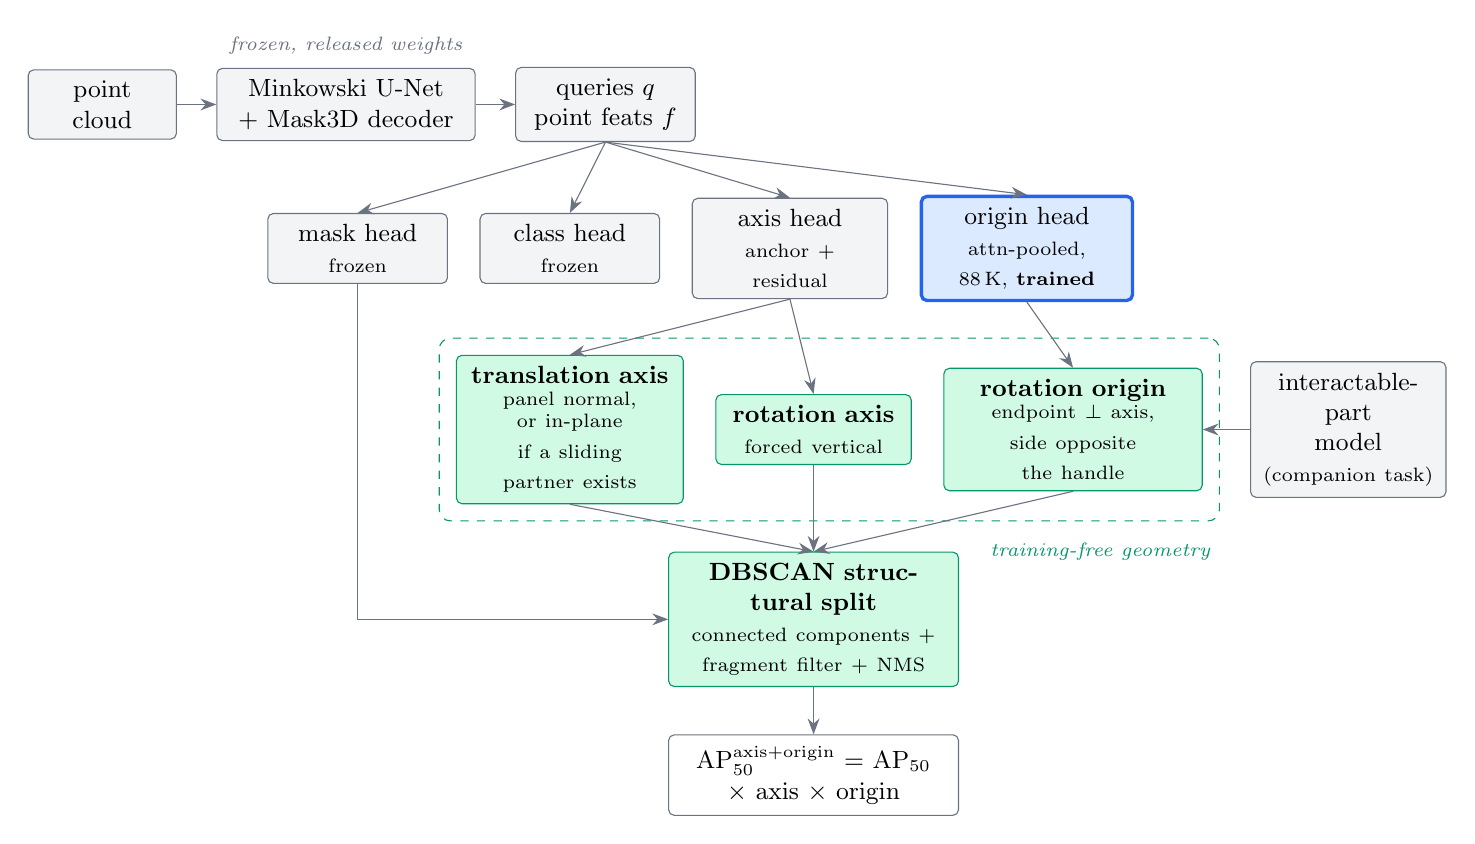
\begin{tikzpicture}[
  font=\small,
  box/.style={draw, rounded corners=2pt, align=center, inner sep=4pt,
              minimum height=8mm, text width=#1},
  froznode/.style={box=#1, fill=froz, draw=frozengray},
  trainode/.style={box=#1, fill=trai, draw=trainedblue, very thick},
  geonode/.style={box=#1, fill=geob, draw=geogreen},
  ar/.style={-{Stealth[length=2mm]}, draw=frozengray},
  lbl/.style={font=\scriptsize\itshape, text=frozengray},
]
\node[froznode=16mm] (pc) {point\\cloud};
\node[froznode=30mm, right=5mm of pc] (bb) {Minkowski U-Net\\ $+$ Mask3D decoder};
\node[froznode=20mm, right=5mm of bb] (feat) {queries $q$\\ point feats $f$};
\draw[ar] (pc) -- (bb); \draw[ar] (bb) -- (feat);
\node[lbl, above=0.5mm of bb] {frozen, released weights};
\node[froznode=20mm, below left=9mm and 20mm of feat.south] (mh) {mask head\\\scriptsize frozen};
\node[froznode=20mm, right=4mm of mh] (ch) {class head\\\scriptsize frozen};
\node[froznode=22mm, right=4mm of ch] (ah) {axis head\\\scriptsize anchor $+$ residual};
\node[trainode=24mm, right=4mm of ah] (oh) {origin head\\\scriptsize attn-pooled, 88\,K, \textbf{trained}};
\foreach \n in {mh,ch,ah,oh} \draw[ar] (feat.south) -- (\n.north);
\node[geonode=26mm, below=9mm of ch] (gtr) {\textbf{translation axis}\\\scriptsize panel normal, or in-plane\\\scriptsize if a sliding partner exists};
\node[geonode=22mm, right=4mm of gtr] (grot) {\textbf{rotation axis}\\\scriptsize forced vertical};
\node[geonode=30mm, right=4mm of grot] (gor) {\textbf{rotation origin}\\\scriptsize endpoint $\perp$ axis,\\\scriptsize side opposite the handle};
\draw[ar] (ah.south) -- (gtr.north); \draw[ar] (ah.south) -- (grot.north); \draw[ar] (oh.south) -- (gor.north);
\node[froznode=22mm, right=6mm of gor] (hnd) {interactable-part\\model\\\scriptsize (companion task)};
\draw[ar] (hnd.west) -- (gor.east);
\begin{scope}[on background layer]
  \node[fit=(gtr)(grot)(gor), draw=geogreen, dashed, rounded corners, inner sep=6pt] (geobox) {};
\end{scope}
\node[lbl, text=geogreen, anchor=north east] at ([yshift=-1.5mm]geobox.south east) {training-free geometry};
\node[geonode=34mm, below=11mm of grot] (dbs) {\textbf{DBSCAN structural split}\\\scriptsize connected components $+$ fragment filter $+$ NMS};
\draw[ar] (gtr.south) -- (dbs.north); \draw[ar] (grot.south) -- (dbs.north); \draw[ar] (gor.south) -- (dbs.north);
\draw[ar] (mh.south) |- (dbs.west);
\node[box=34mm, below=6mm of dbs, draw=frozengray, fill=white] (out) {\metric{} $=$ \apfifty{} $\times$ axis $\times$ origin};
\draw[ar] (dbs) -- (out);
\end{tikzpicture}
\caption{\textbf{Method overview.} Grey: frozen at released weights. Blue: the only trained component. Green: training-free geometry read off the predicted masks and the offline structural post-processing.}
\label{fig:recipe}
\end{figure}

\section*{Results (challenge server, ranking metric)}
\begin{center}
\small
\begin{tabular}{@{}lcc@{}}
\toprule
Configuration (cumulative) & Movable test \metric{} & Interaction test \apfifty{} \\
\midrule
USDNet baseline (reproduced) & 0.2640 & 0.2686 \\
$+$ trained origin head $+$ geometric priors & 0.3385 & --- \\
$+$ DBSCAN structural post-processing & 0.3760 & 0.2886 \\
$+$ flip finetune / ensemble (final) & \textbf{0.4056} & \textbf{0.3286} \\
\midrule
Relative to baseline & $+54\%$ & $+22\%$ \\
\bottomrule
\end{tabular}
\end{center}

\end{document}
